%%%%%%%%%%%%%%%%%%%%%%%%%%%%%%%%%%%%%%
% Contribution to IKP annual report 2018
%%%%%%%%%%%%%%%%%%%%%%%%%%%%%%%%%%%%%%
\documentclass[fleqn,twocolumn,a4paper]{ikpar}
\usepackage{hyperref}
\usepackage{paralist}
\usepackage{times,mathptm}
\usepackage{graphicx}
\usepackage{caption}
\usepackage{subfig}
\usepackage{gensymb}
\pagestyle{empty}

% standadized SI units
\usepackage[per-mode=symbol, range-units=single, binary-units=true]{siunitx}
\DeclareSIUnit\clight{\text{\ensuremath{c}}} % redefine light speed symbol
\DeclareSIUnit\momentum{\GeV\per\clight} % momentum in GeV/c
\DeclareSIUnit\tmom{(\momentum)^2} % 4-momentum squared
\DeclareSIUnit\atom{\text{atoms}} 
\DeclareSIUnit\event{\text{events}} 

% \addtolength{\topmargin}{-0.2cm}
% \addtolength{\textheight}{0.2cm}
\begin{document}
\parindent=0pt
\frenchspacing

\title{{\bf
    Determination of the cluster target density profile in KOALA
}}
\author{Yong Zhou
  and Huagen Xu
}

\maketitle

%%%% Background, problem description, topic and results of this report
KOALA aims to achieve measure the differential cross section of $pp$ elastic
scattering over a wide $|t|$ range \SIrange{0.0008}{0.1}{tmom}.
The forward detector, which is made from fast scintillators, has been built to help
supressing the low energy background at small recoil angle by coincidence
measurement with the recoil detector.
The design of the forward detector is verified in these tests and the elastic
events are correctly identified from large backgrounds.
However, it is also found that the size of the cluster target can't be
neglected at very small recoil angles and the elastic energy spectrum is
deterioated by the density distribution of the target profile.
Thus, an accurate information about the target density distribution is needed to exact
the elastic peak correctly.
A method for the determination of the cluster target density profile from the
test beam data is developped for this purpose.
\par
\medskip

%%%%% Description of the method
The number of elastic events $N_{evt}$ recorded in the experiment follows the
equation $N_{evt} =
l_{beam}\cdot\rho_{target}\cdot\sigma_{elastic}\cdot\epsilon_{acceptance}\cdot\epsilon_{detection}$,
where $l_{beam}$ is beam intensity, $\rho_{target}$ is the target density,
$\sigma_{elastic}$ is the cross section of elastic scattering,
$\epsilon_{acceptance}$ and $\epsilon_{detection}$ are the detector acceptance
and the combined
detection efficiency of the detectors and DAQ.
$l_{beam}$ and $\epsilon_{detection}$ are constant parameters in the same run.
To determine the target density, a reference in which $\sigma_{elasitc}$ and
$\epsilon_{acceptance}$ are both invariate is needed.
% The event count in the same energy bin close to the lower edge of the forward
% fully-covered region is selected as the reference for the density determination.
Fig. \ref{fig:spectrums} shows the elastic energy spectrums recorded by different strips of Si1 at beam momentum \SI{2.2}{\momentum}.
The observed lower edge of the forward acceptance is about \SI{100}{\keV} while the
trigger threshold is about \SI{50}{\keV}.
The lower edge is in accordance with the calculated range of the
fully-covered recoil energy by the forward detector at \SI{2.2}{\momentum},
which is \SIrange{0.096}{1.56}{\MeV}.
Due to the full coverage, the event counts in the energy bin close to the lower edge (for example
\SI{120}{\keV}) acts as the meter of the target density at the position
corresponding to this energy bin.
Since strips are located along the beam axis, both before and after the target
chamber center, the aggregation of the measurements on all the strips provide a full scan of the target denstiy profile along the beam axis.
The strips are organized into two groups in Fig. \ref{fig:spectrums}: 1) the
target peak density is not covered by the strips
before Si1\_18 and they measures the target profile before the peak density; 2) the target
peak gradually shows up on strips after Si1\_18 and they measures the profile
after the peak density.

\begin{figure}[!htb]
	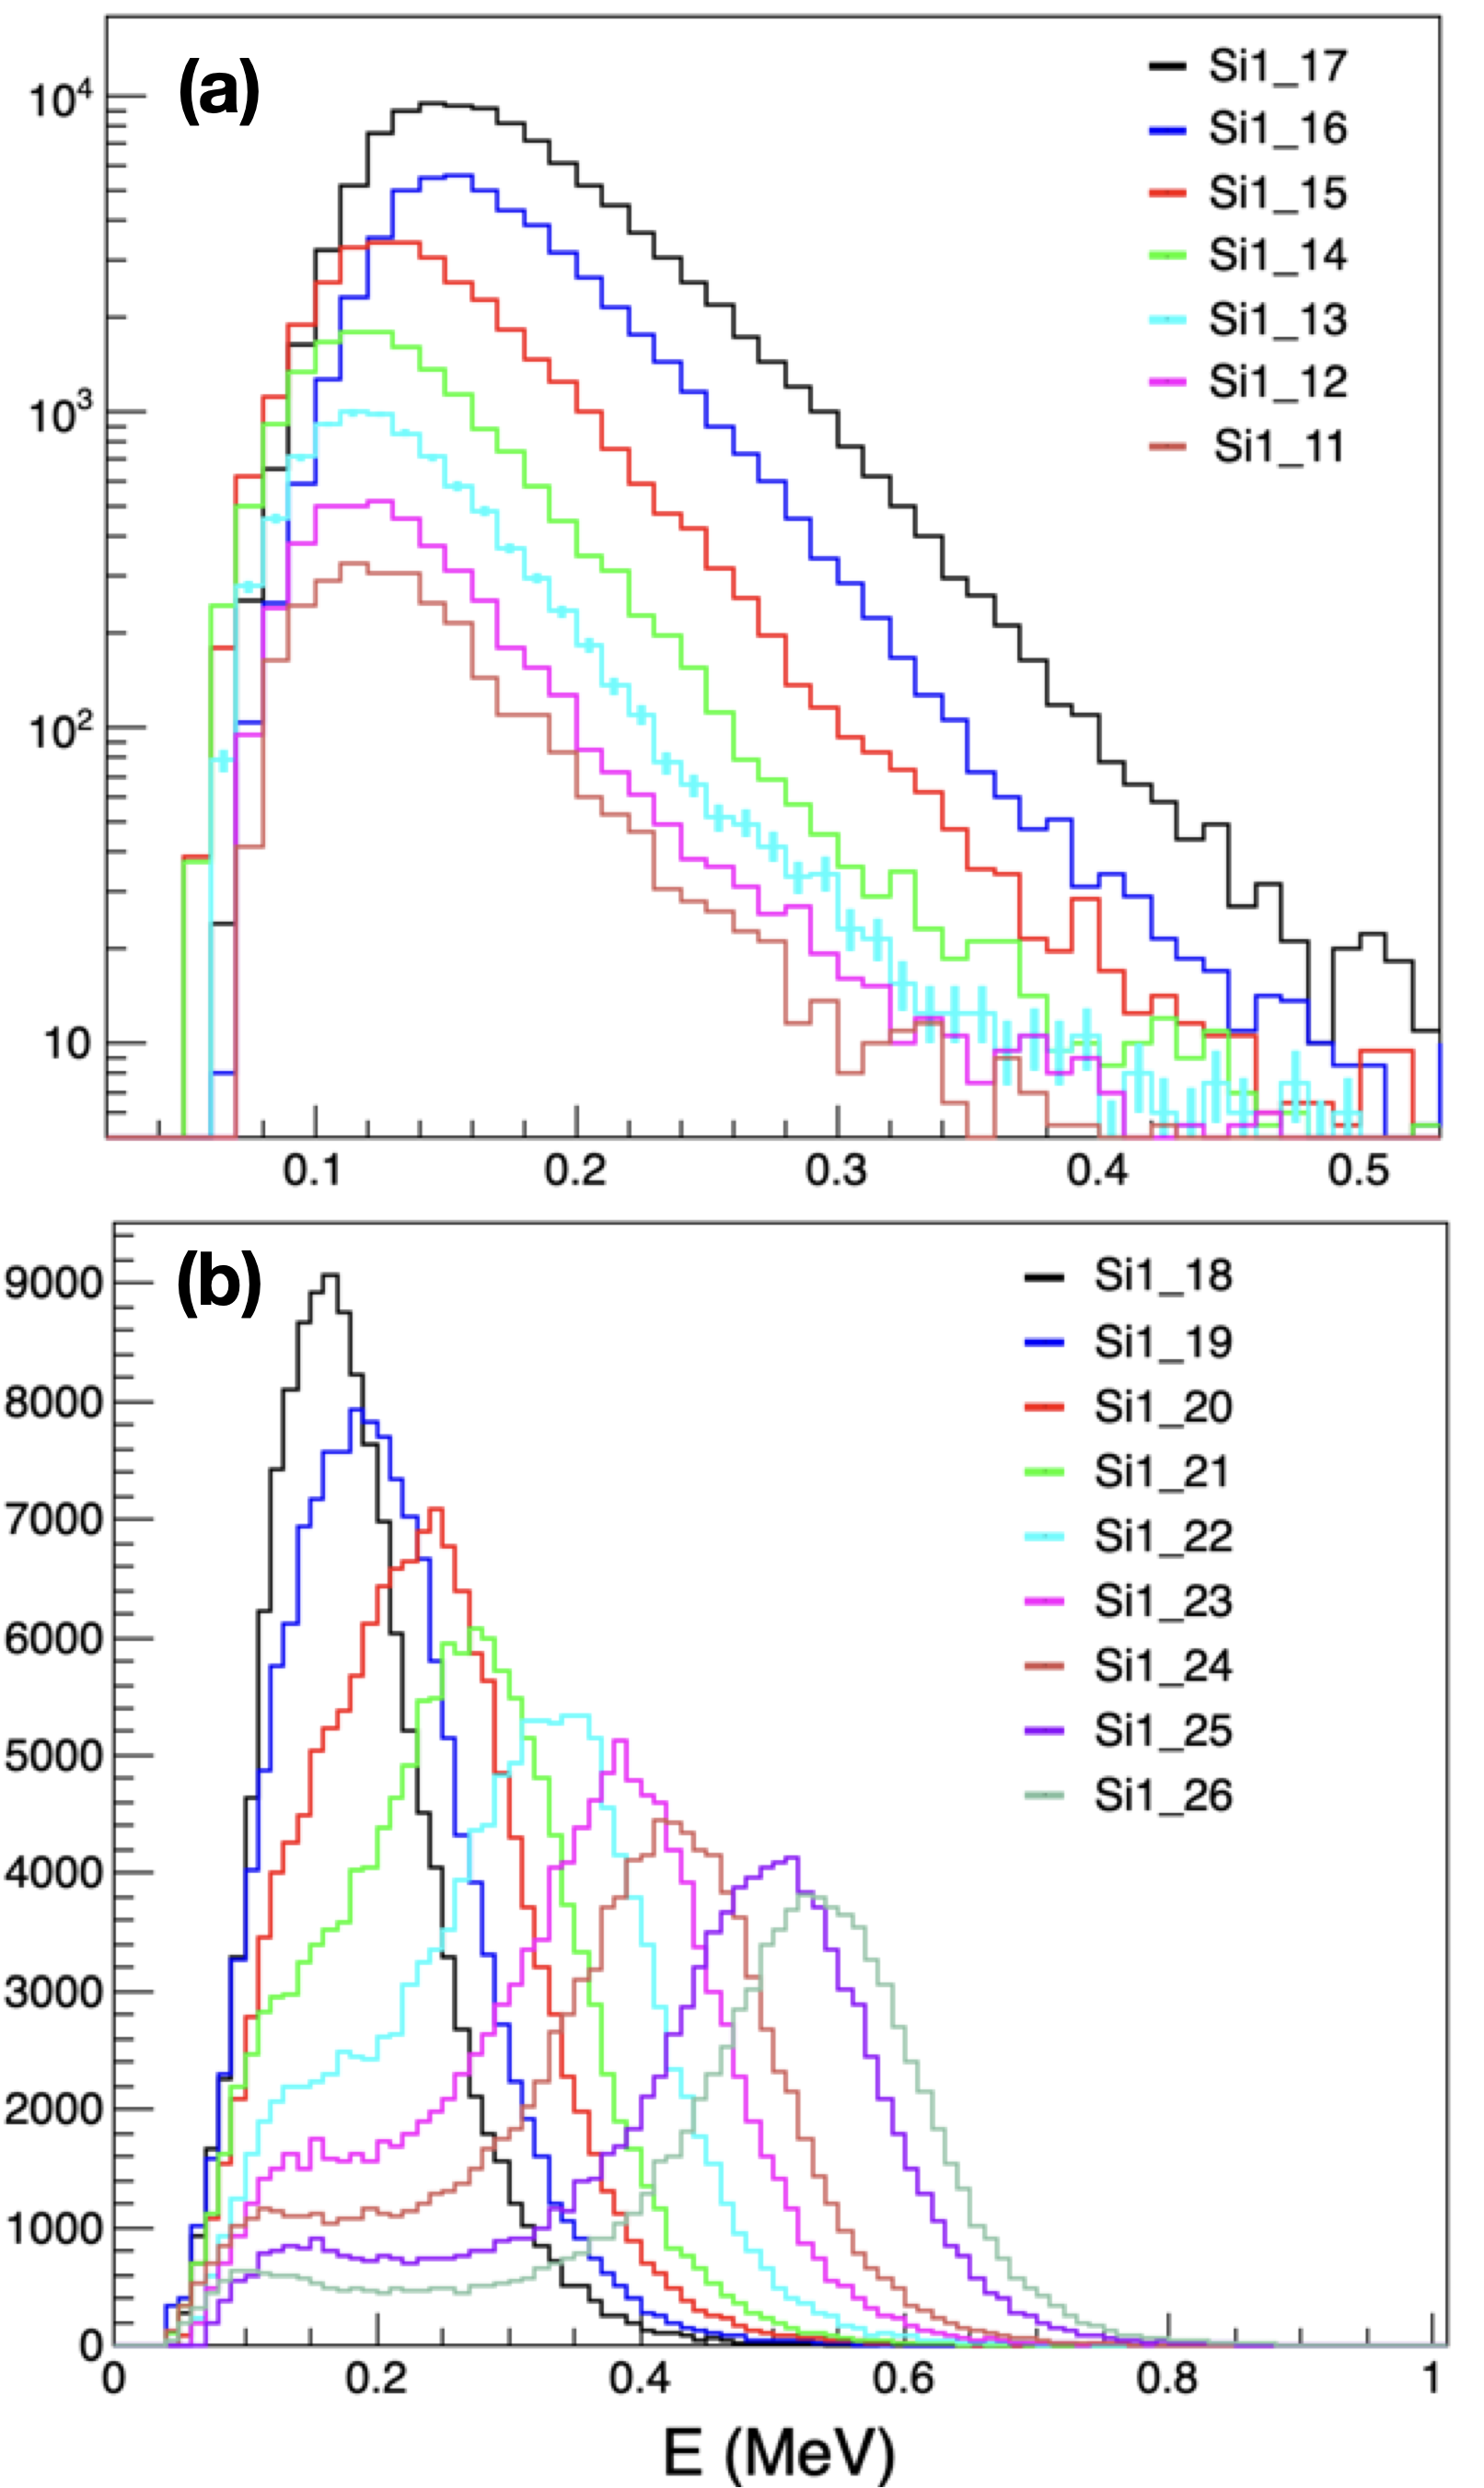
\includegraphics[width=0.5\textwidth]{./spectrums_aggregate.png}
  	\caption{Key steps, important classes and the data flow in \textbf{unpack} package}
  	\label{fig:unpack_design}
\end{figure}

%%%%% Results of the method
Two independent methods can be used to determine the position distribution of the density profile.
The first method is based on the strip position of the ideal geometry model.
The reference energy bin is convered to a position before the strip center (for
\SI{120}{\keV}, it converts to \SI{10}{\mm} at \SI{2.2}{\momentum}), which in turn
gives the absolute position of this profile slice in the reference frame of the
ideal geometry model.
The second method is based on the energy difference of the reference energy bin
and the elastic peak.
The elastic energy peak corresponds to the target density peak.
The energy difference can be converted to the relative position of this profile
slice against the target profile peak.
This method is limited by the coverage of the elastic and only gives the density distribution after the target peak.
The comparison between these two results is used to align the the recoil
detector to the target center.
\par
\medskip

%%%%% Discussion of the results
Fig. \ref{fig:result} shows the target density profile measured at
\SI{2.2}{\momentum}.
The target density is almost symmetric against the peak value.
The main body of the target is fitted with a double-gaussian, in which the
narrow component has $\sigma$ of \SI{2}{mm} and the wide one has $\sigma$ of \SI{5.6}{mm}.
The overall FWHM of the target distribution is about \SI{6.9}{mm}.
A flat residual gas distribution over a wide region is also observed.
Although the dendity of the residual gas is about 200x lower than the peak
value, they introduce an unnegligible elastic background at small recoil angle.

The measured target density distribution is wider than required design value and
explains the deteriation observed at small recoil angles.
With the newly measured target density profile, it's now possible to unfold the the
measured spectrum at very small recoil angles.
This opens the possibility of extending the range of measurable $|t|$ to a lower limit.

\par
\medskip

%----------------------------------------------------------------
\begin{thebibliography}{99}
\bibitem{r1} \url{https://github.com/FairRootGroup/FairRoot}
\bibitem{r2} Y. Zhou, H. Xu, IKP Annual Report 2018
\bibitem{r3} K. H. Watzlawik et al. IEEE Transactions on Nuclear Science 43 (1996): 44
\bibitem{r4} \url{https://root.cern.ch}
\end{thebibliography}
\end{document}

